\documentclass[a4paper,UTF8]{article}
\usepackage{ctex}
\usepackage[margin=1.25in]{geometry}
\usepackage{color}
\usepackage{graphicx}
\usepackage{amssymb}
\usepackage{amsmath}
\usepackage{amsthm}
\usepackage{soul, color, xcolor}
\usepackage{bm}
\usepackage{tcolorbox}
\usepackage{hyperref}
\numberwithin{equation}{section}
%\usepackage[thmmarks, amsmath, thref]{ntheorem}
\theoremstyle{definition}
\newtheorem*{solution}{Solution}
\newtheorem*{prove}{Proof}
\usepackage{multirow}
\usepackage{diagbox}
\usepackage{float}

\def \X {\mathbf{X}}
\def \W {\mathbf{W}}
\def \A {\mathbf{A}}
\def \K {\mathbf{K}}
\def \B {\mathbf{B}}
\def \C {\mathbf{C}}
\def \Q {\mathbf{Q}}
\def \S {\mathbf{S}}
\def \P {\mathbf{P}}
\def \Diag {\textbf{$\Lambda$}}
\def \w {\hat{\boldsymbol{w}}}
\def \y {\boldsymbol{y}}
\def \x {\boldsymbol{x}}
\def \z {\mathbf{z}}
\def \b {\mathbf{b}}
\def \by {\Bar{y}}
\def \H {\mathbf{H}}
\def \I {\mathbf{I}}
\setlength{\parindent}{0pt}
%--

%--
\begin{document}
\title{机器学习导论\ 习题三}
\author{221300079, 王俊童, \href{mailto:221300079@smail.nju.edu.cn}{221300079@smail.nju.edu.cn}}
\maketitle
\section*{作业提交注意事项}
\begin{tcolorbox}
	\begin{enumerate}
    \item[1.] 作业所需的LaTeX及Python环境配置要求请参考: \href{https://www.lamda.nju.edu.cn/ML2024Spring/supplemantary/environment.pdf}{[Link]};
		\item[2.] 请在LaTeX模板中第一页填写个人的学号、姓名、邮箱;
		\item[3.] 本次作业需提交的文件与对应的命名方式为:
            \begin{enumerate}
                \item [(a)] 作答后的LaTeX代码 --- \texttt{HW3.tex};
                \item [(b)] 由(a)编译得到的PDF文件 --- \texttt{HW3.pdf};
                \item [(c)] 第三题模型代码 --- \texttt{p3\_models.py};
                \item [(d)] 第四题模型代码 --- \texttt{p4\_models.py};
                \item [(e)] 第四题训练代码 --- \texttt{p4\_trainer.py}.
            \end{enumerate}
            请将以上文件{\color{red}\textbf{打包为~学号\hspace{0em}\_\hspace{0em}姓名.zip}} (例如 221300001\hspace{0em}\_\hspace{0em}张三.zip) 后提交;
		\item[3.] 若多次提交作业, 则在命名~.zip 文件时加上版本号, 例如 221300001\_\hspace{0em}张三\hspace{0em}\_v1.zip” (批改时以版本号最高的文件为准);
		\item[4.] 本次作业提交截止时间为 {\color{red}\textbf{ 5 月 17 日23:59:59}}. 未按照要求提交作业, 提交作业格式不正确, {\color{red}\textbf{作业命名不规范}}, 将会被扣除部分作业分数; 除特殊原因 (如因病缓交, 需出示医院假条) 逾期未交作业, 本次作业记 0 分; {\color{red}\textbf{如发现抄袭, 抄袭和被抄袭双方成绩全部取消}};
        \item[5.] 学习过程中, 允许参考 ChatGPT 等生成式语言模型的生成结果, 但必须在可信的信息源处核实信息的真实性; {\color{red}\textbf{不允许直接使用模型的生成结果作为作业的回答内容}}, 否则将视为作业非本人完成并取消成绩;
		\item[6.] 本次作业提交地址为 \href{https://box.nju.edu.cn/u/d/cf36400095e94f769e1d/}{[Link]}, 请大家预留时间提前上交, 以防在临近截止日期时, 因网络等原因无法按时提交作业.
	\end{enumerate}
\end{tcolorbox}
\newpage

    %\begin{figure}[H]
    %    \centering
    %    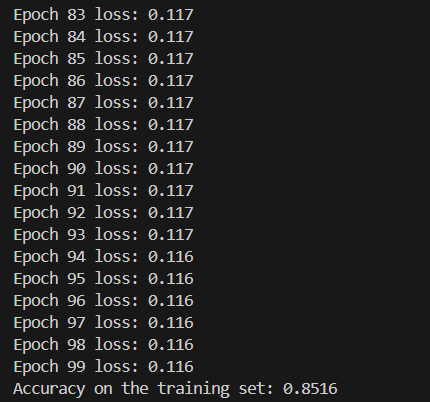
\includegraphics[width=1\textwidth]{4.png}\\
    %    \caption{Unraveling graph}
    %    \label{fig:Unraveling}
    %\end{figure}  


\section{[25pts] Principal Component Analysis}
主成分分析是一种经典且常用的数据降维方法. 请仔细阅读学习《机器学习》第十章 10.3 节, 并根据图 10.5 中的算法内容, 完成对如下 6 组样本数据的主成分分析. 
        \[
        \X = \begin{bmatrix}
            2&3&3&4&5&7\\
            2&4&5&5&6&8
        \end{bmatrix}
        \]
        
\begin{enumerate}
    \item[(1)] \textbf{[6pts]} 试求样本数据各维的均值、标准差.
    \item[(2)] \textbf{[7pts]} 试求标准化后的样本矩阵 $\X_{\text{std}}$, 以及 $\X_{\text{std}}$ 对应的协方差矩阵.
    \item[(3)] \textbf{[7pts]} 试求协方差矩阵对应的特征值, 以及投影矩阵 $\W^\star$. 
    \item[(4)] \textbf{[5pts]} 如果选择重构阈值 $t=95\%$, 试求 PCA 后样本 $\X_{\text{std}}$ 在新空间的坐标矩阵.
\end{enumerate}

 

\begin{solution} 
    (1)因为这里有6组样本\\
    对于每组数据内部来说,均值为$2,3.5,4,4.5,5.5,7.5$\\
    对于每组数据来说(每行),均值为$4,5$\\
    根据标准差计算公式:$\sigma = \sqrt[]{\frac{\sum_{1}^{n}X - X_{mean}}{n}}$\\
    对于每组数据内部来说,标准差为$0,0.5,1,0.5,0.5,0.5$\\
    对于每组数据来说(每行),标准差为约$1.63,1.83$\\
    (2)对于标准化数据来说,按照公式计算可得约为:$X_{new} = \frac{X - \mu}{\sigma}$\\
    \[
        \X = \begin{bmatrix}
            -1.225&-0.612&-0.612&0&0.612&1.837\\
            -1.643&-0.548&0&0&0.548&1.643
        \end{bmatrix}
    \]
    所以可计算协方差约为:$Cov = \frac{1}{n-1} X^T *X$\\
    \[
        \mathbf{Cov} = \begin{bmatrix}
            1.20&1.14\\
            1.14&1.20
        \end{bmatrix}
    \]
    (3).可以求特征值为:$\mathbf{Cov} - \lambda \mathbf{I} = 0$,解得约为:$\lambda_1 = 2.34, \lambda_2 = 0.06$.\\
    带入原式子进行求解,可以得到标准化后的特征向量:\\
    \[
        \mathbf{Eigenvector} = \begin{bmatrix}
            0.707&-0.707\\
            0.707&0.707
        \end{bmatrix}
    \]
    所以投影矩阵根据规则可以选择为:\\
    \[
        \mathbf{W^*} = \begin{bmatrix}
            0.707\\
            0.707
        \end{bmatrix}
    \]
    (4).由于根据书上所说,$\frac{\sum_{i=1}^{d'}\lambda_i}{\sum_{i=1}^{d}\lambda_i} \geq t$,这个意思跟pca中的$n\_Component$是一个意思,我们可以有刚刚计算出的标准化后的
    矩阵乘上$W^*$可以得到:\\
    \[
        \mathbf{X_{pca}} = \begin{bmatrix}
            -2.028\\
            -0.820\\
            -0.431\\
            0\\
            0.820\\
            2.461
        \end{bmatrix}
    \]
    所以新空间坐标矩阵即为所求.
\end{solution}


\newpage
\section{[25pts] Support Vector Machines}
核函数是 SVM 中常用的工具,其在机器学习中有着广泛的应用与研究. 请仔细阅读学习《机器学习》第六章, 并回答如下问题.
\begin{enumerate}
	\item[(1)] \textbf{[6pts]} 试判断下图 $\textcircled{1}$ 到 $\textcircled{6}$ 中哪些为支持向量.
        \begin{figure}[!htbp]
		\centering
			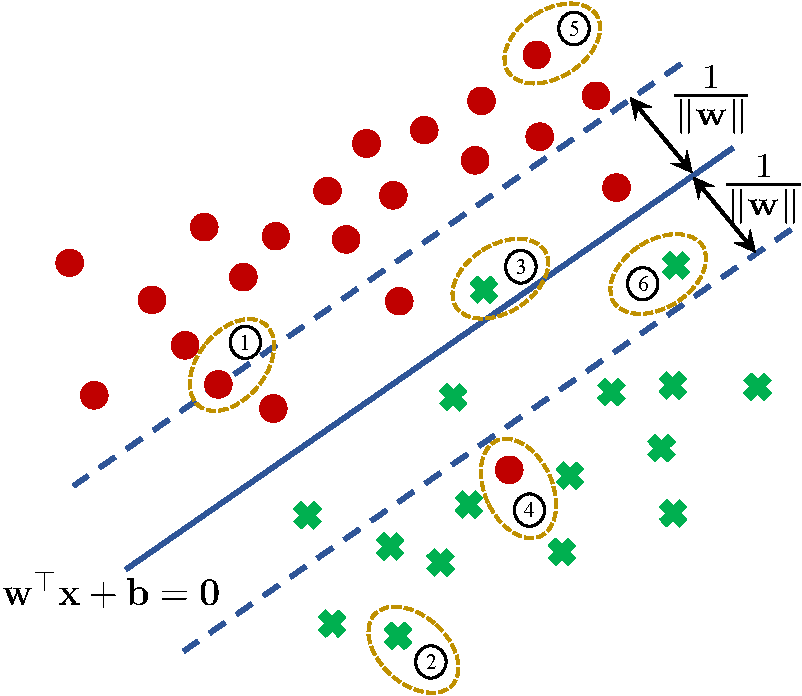
\includegraphics[width=0.48\textwidth]{svm.pdf}\\
			\caption{分离超平面示意图}
	\end{figure}
        \item[(2)] \textbf{[5pts]} 试判断 $\kappa(\x, \z) = \left(\langle\x, \z\rangle + 1\right)^2$ 是否为核函数,并给出证明或反例.
        \item[(3)] \textbf{[5pts]} 试判断 $\kappa(\x, \z) = \left(\langle\x, \z\rangle - 1\right)^2$ 是否为核函数,并给出证明或反例.
	\item[(4)] \textbf{[9pts]} 试证明:若 $\kappa_1$ 和 $\kappa_2$ 为核函数, 则两者的直积
	\[
	\kappa_1 \otimes \kappa_2(\x, \z)=\kappa_1(\x, \z) \kappa_2(\x, \z)
	\]
	也是核函数. 即证明 《机器学习》(6.26) 成立.

 (\textbf{Hint:} 利用核函数与核矩阵的等价性.)

	
\end{enumerate}

\begin{solution}
(1).根据支持向量的定义,可以得到,需要找到离平面最近的点,且满足以下条件的等式形式:
\begin{equation*}
    \begin{cases}
        w^T x_i + b \geq 1 & y_i = + 1\\
        w^T x_i + b \leq 1 & y_i = -1
    \end{cases}
\end{equation*}
可得:点1是满足条件的支持向量\\
(2).是核函数,下面给出证明\\
证明:$y^T \mathbf{K} y \geq 0$\\
对于$K_{ij} = \kappa(x_i,x_j) = <x_i,x_j>^2 + 2<x_i,x_j> + 1 $
所以我们可以得到:\\
$y^T \mathbf{K} y = \sum_{i=1}^{j} \sum_{j=1}^{n} y_i y_j *(<x_i,x_j>^2 + 2<x_i,x_j> + 1)\\
= \sum_{i=1}^{j} \sum_{j=1}^{n}( y_i y_j <x_i,x_j>^2) + \sum_{i=1}^{j} \sum_{j=1}^{n}( y_i y_j 2<x_i,x_j>) + \sum_{i=1}^{j} \sum_{j=1}^{n}( y_i y_j ) $
对于这个式子的第一个项,显然是大于等于0的\\
对于这个式子的第二个项,这是一个线性核函数演化成的,所以合法\\
对于第三项,显然也是非负的\\
所以综上可以得到这个核函数是非负的。\\

(3).不是核函数,可以给出一个反例如下:$(0,1),(1,0)$\\
对于这个东西的核矩阵我们可以得到:\\
\[\begin{bmatrix}
    0 & 1\\
    1 & 0
\end{bmatrix}\]
对于这个矩阵,并不是半正定的,所以这个不是核函数。

(4).由于根据书上所说:$k_1 \otimes k_2(x,z) = k_1(x,z) k_2(x,z)$,下面给出证明:\\
首先我们令$K = k_1 \otimes k_2, K_1 = k_1(x,z), K_2 =  k_2(x,z)$\\
根据mercer定理,我们可以得知,只要证明了这个K是半正定的,我们即可证明这个式子成立,已知,$K_1,K_2$都是半正定的,而且满足核函数和核矩阵的等价概念:\\
所以,给出:\\
$y^T K y  = y^T 
\begin{bmatrix}
    k_1(x_1,z_1) k_2(x_1,z_1) & ... &  k_1(x_1,z_n) k_2(x_1,z_n)\\
    ... & ... & ...\\
    k_1(x_n,z_1) k_2(x_n,z_1) & ... &  k_1(x_n,z_n) k_2(x_n,z_n)
\end{bmatrix}y
= \sum_{i=1}^{n}\sum_{j=1}^{n} k_1(x_i,z_j) k_2(x_i,z_j) y_i y_j \\
\\
= tr (
\begin{bmatrix}
    y_1 k_1(x_1,z_1) & ... & ... & ...\\
    ... & y_2 k_1(x_2,z_2) & ... & ...\\
    ... & ... & ... & ... \\
    ... & ... & ... & y_n k_1(x_n,z_n)\\
\end{bmatrix}
\begin{bmatrix}
    y_1 k_2(x_1,z_1) & ... & ... & ...\\
    ... & y_2 k_2(x_2,z_2) & ... & ...\\
    ... & ... & ... & ... \\
    ... & ... & ... & y_n k_2(x_n,z_n)\\
\end{bmatrix})
$
我们已经知道了,对于两个k矩阵,他们是核函数,所以他们的核矩阵也是半正定的,所以我们可以得到:$K_1 = A^T A, K_2 = B^T B$,带入可得\\
$
=tr (
\begin{bmatrix}
    y_1 & ... & ... & ...\\
    ... & y_2 & ... & ...\\
    ... & ... & ... & ... \\
    ... & ... & ... & y_n \\
\end{bmatrix}A^T A
\begin{bmatrix}
    y_1 & ... & ... & ...\\
    ... & y_2 & ... & ...\\
    ... & ... & ... & ... \\
    ... & ... & ... & y_n \\
\end{bmatrix}
B^T B )\\
\\
= tr (B
\begin{bmatrix}
    y_1 & ... & ... & ...\\
    ... & y_2 & ... & ...\\
    ... & ... & ... & ... \\
    ... & ... & ... & y_n \\
\end{bmatrix}A^T 
A
\begin{bmatrix}
    y_1 & ... & ... & ...\\
    ... & y_2 & ... & ...\\
    ... & ... & ... & ... \\
    ... & ... & ... & y_n \\
\end{bmatrix}
B^T)\\
\\
=  tr ((A
\begin{bmatrix}
    y_1 & ... & ... & ...\\
    ... & y_2 & ... & ...\\
    ... & ... & ... & ... \\
    ... & ... & ... & y_n \\
\end{bmatrix}B^T)^T 
(A
\begin{bmatrix}
    y_1 & ... & ... & ...\\
    ... & y_2 & ... & ...\\
    ... & ... & ... & ... \\
    ... & ... & ... & y_n \\
\end{bmatrix}
B^T))\\
\\
= tr(P^T P) \geq 0
$\\
所以我们即通过核矩阵证明了这个定理是成立的,这个矩阵半正定

\end{solution}

\newpage

\section{[30pts] Basics of Neural Networks}

多层前馈神经网络可以被用作分类模型. 在本题中, 我们先回顾前馈神经网络的一些基本概念, 再利用 Python 实现一个简单的前馈神经网络以进行分类任务.

\textbf{[基础原理]} 首先, 考虑一个多层前馈神经网络, 规定网络的输入层是第 $0$ 层, 输入为 $\mathbf{x} \in \mathbb{R}^d$. 网络有 $M$ 个隐层, 第 $h$ 个隐层的神经元个数为 $N_h$, 输入为 $\mathbf{z}_h\in \mathbb{R}^{N_{h-1}}$, 输出为 $\mathbf{a}_h \in \mathbb{R}^{N_h}$, 权重矩阵为 $\mathbf{W}_h \in \mathbb{R}^{N_{h-1} \times N_{h}}$, 偏置参数为 $\mathbf{b}_h \in \mathbb{R}^{N_h}$. 网络的输出层是第 $M+1$ 层, 神经元个数为 $C$, 权重矩阵为 $W_{M+1} \in \mathbb{R}^{N_M \times C}$, 偏置参数为 $\mathbf{b}_{M+1} \in \mathbb{R}^C$, 输出为 $\mathbf{y} \in \mathbb{R}^C$. 网络隐层和输出层的激活函数均为 $f$, 网络训练时的损失函数为 $\mathcal{L}$, 且 $f$ 与 $\mathcal{L}$ 均可微.

\begin{enumerate}
    \item [(1)] \textbf{[5pts]} 请根据前向传播原理, 给出 $\mathbf{z}_h, \mathbf{a}_h\ (1\leq h \leq M)$ 及 $\mathbf{y}$ 的具体数学表示.
    \item [(2)] \textbf{[5pts]} 结合 (2) 的表示形式, 谈谈为何要在神经网络中引入 (非线性) 激活函数 $f$?
\end{enumerate}

\textbf{[编程实践]} 下面, 我们针对一个特征数 $d=2$, 类别数为 $2$ 的分类数据集, 实现一个结构为 ``2-2-1'' 的简单神经网络, 即: 输入层有 $2$ 个神经元; 隐层仅一层, 包含 $2$ 个神经元; 输出层有 $1$ 个神经元; 所有层均使用 Sigmoid 作为激活函数. 此外, 我们使用 BP 算法进行神经网络的训练. \textbf{关于本题的细节介绍及具体要求, 请见附件: \href{https://www.lamda.nju.edu.cn/ML2024Spring/homework/HW3/p3_guide.pdf}{\texttt{p3\hspace{0em}\_\hspace{0em}编程题说明}}.} 请参考编程题说明文档与附件中的代码模板, 完成下面的任务.

\begin{enumerate}
    \item [(3)] \textbf{[15pts]} 基于 \texttt{p3\_models.py}, 补全缺失代码, 实现神经网络分类器的训练与预测功能.
    \item [(4)] \textbf{[5pts]} 参考《机器学习》及第一次作业中对超参数调节流程的介绍, 为 (1) 中模型设置合适的超参数 (即: 学习率与迭代轮数). \textbf{请将选择的超参数设置为调用模型时的默认参数, 并在解答区域简要介绍你的超参数调节流程.}\\(提示: 可以从数据集划分方法, 评估方法, 候选超参数生成方法等角度说明).
\end{enumerate}

\begin{solution} 
(1).
结合书上的推导可以得到,假如偏置常数在这里得到的是阈值:\\
$
\mathbf{z_h} = \mathbf{a_{h-1}} \mathbf{W_h} \\
\mathbf{a_h} = f(\mathbf{z_h} +  \mathbf{b_h})\\
\mathbf{y} = f(\mathbf{a_M}\mathbf{W_{h+1}} + \mathbf{b_{M-1}})
$.

(2).关于引入非线性激活函数可以从以下几个方向考虑:\\
1.非线性激活函数表达力相比线性函数更强,线性函数容易出现多层神经网络之后的梯度消失问题,非线性函数这种方式可以使得神经网络学到复杂的函数映射关系,从而有万有逼近性。\\
2.非线性激活函数可以实现非线性可分数据的判别,可以解决复杂的数据分布。\\
3.可以增强模型的学习能力和泛化能力,网络可以学习更为复杂的模型,还可以控制防止过拟合。\\
4.有助于梯度传播和反向传播,梯度传播和反向传播需要激活函数的存在来实现。激活函数的导数可以帮助计算每一层的梯度,并在反向传播过程中传递误差信号,从而更新网络参数。\\

(3).我已经实现了10轮的基本训练,在学习率为给定的0.01的情况下,我的神经网络做到了以下效果:\\
\begin{figure}[H]
    \centering
    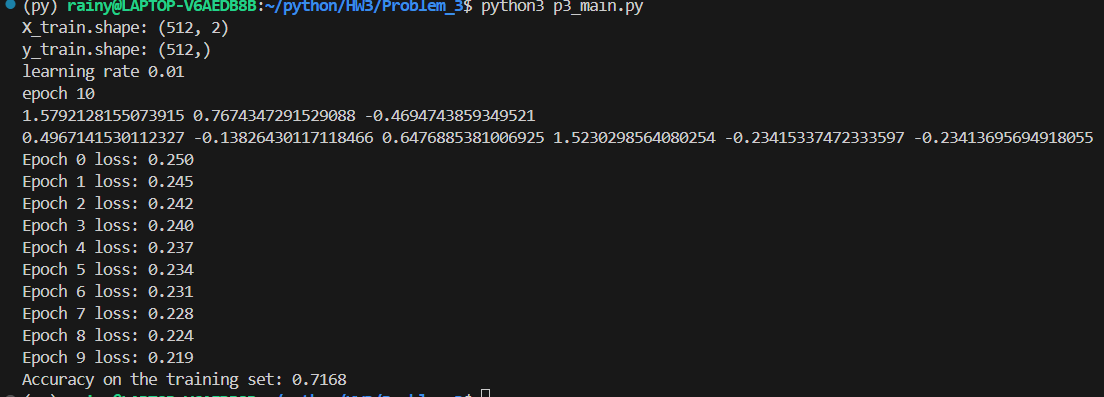
\includegraphics[width=0.75\textwidth]{3.png}\\
    \caption{NN with 10 epoch, 0.01 lr}
    \label{fig:NN with 10 epoch, 0.01 lr}
\end{figure}  

(4)调节超参数:\\
方法一:在现有学习率下面增大轮数:我们把epoch搞到100轮\\
\begin{figure}[H]
    \centering
    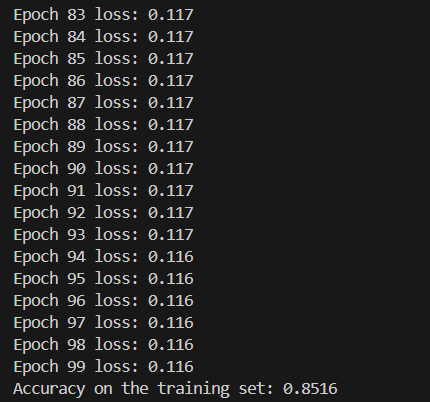
\includegraphics[width=0.75\textwidth]{4.png}\\
    \caption{NN with 100 epoch, 0.01 lr}
    \label{fig:NN with 100 epoch, 0.01 lr}
\end{figure}  
梯度下降到了0.116左右,而且准确率高达0.8516\\
方法二:现有梯度下,调整一下学习率,这个我们发现学习率越大,效果越好,我们调整到0.05-0.1左右:\\
\begin{figure}[H]
    \centering
    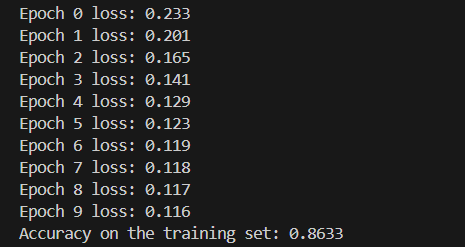
\includegraphics[width=0.75\textwidth]{5.png}\\
    \caption{NN with 10 epoch, 0.07 lr}
    \label{fig:NN with 10 epoch, 0.07 lr}
\end{figure} 
方法三,都做调整\\
\begin{figure}[H]
    \centering
    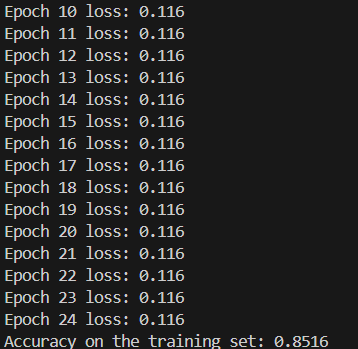
\includegraphics[width=0.5\textwidth]{6.png}\\
    \caption{NN with 25 epoch, 0.07 lr}
    \label{fig:NN with 25 epoch, 0.07 lr}
\end{figure} 
可以看出在这个情况下,其实差距都不大,而且经过多次调试比如100epoch,0.1的lr我发现这个梯度下降至0.116附近就不动了,但也不一定说明
全局最优就是这个点,有可能这是个局部最优,所以对于这个问题目前就这样。


\end{solution}

\newpage

\section{[20(+5)pts] Neural Networks with PyTorch}

\begin{tcolorbox}
在上一题的编程实践中, 我们使用 Python 实现了一个简单的神经网络分类器. 其中, 我们根据 BP 算法中神经网络参数梯度的数学定义, 手动实现了梯度计算及参数更新的流程. 然而, 在现实任务中, 我们往往利用\textit{深度学习框架}来进行神经网络的开发及训练. 一些常用的框架例如: PyTorch, Tensorflow 或 JAX, 以及国产的 PaddlePaddle, MindSpore. 这类框架往往支持\textit{自动微分}功能, 仅需定义神经网络的具体结果与前向传播过程, 即可在训练时自动计算参数的梯度, 进行参数更新. 此外, 我们可以使用由框架实现的更成熟的优化器 (如 Adam 等) 来提高模型的收敛速度, 或使用 GPU 加速以提高训练效率. 如果希望在今后的学习科研中应用神经网络, 了解至少一种框架的使用方式是极为有益的.
\end{tcolorbox}

在本题中, 我们尝试使用 PyTorch 框架来进行神经网络的开发, 完成 FashionMNIST 数据集上的图像分类任务. 与上一题考察神经网络底层原理不同, 本题考察大家阅读文档, 搭建模型并解决实际任务的能力. \textbf{关于本题的细节介绍及具体要求, 请见附件: \href{https://www.lamda.nju.edu.cn/ML2024Spring/homework/HW3/p4_guide.pdf}{\texttt{p4\hspace{0em}\_\hspace{0em}编程题说明}}.} 请参考编程题说明文档与附件中的代码模板, 完成下面的任务.

\begin{enumerate}
    \item [(1)] \textbf{[10pts]} 阅读文档, 配置 PyTorch 环境, 补全 \texttt{p4\_models.py} 中神经网络的 \texttt{\_\_init\_\_} 与 \texttt{forward} 方法, 最终成功运行 \texttt{p4\_main.py}. \textbf{请在解答区域附上运行 \texttt{p4\_main.py} 后生成的 \texttt{plot.png}.}
    \item [(2)] \textbf{[10pts]} 从 (1) 中生成的训练过程图片 \texttt{plot.png} 中可以看出: 模型明显出现了\textbf{过拟合}现象, 即训练一定轮次后, 训练集 loss 持续下降, 但测试集 loss 保持不变或转为上升. \\请提出\textbf{至少两种}缓解过拟合的方法, 分别通过编程实现后, 在解答区域附上应用前后的训练过程图片, 并结合图片简要分析方法有效/无效的原因.\\(提示: 可以考虑的方法包括但不限于: Dropout, 模型正则化, 数据增强等.)
    \item [(3)] \textbf{[5pts]} (本题为附加题, 得分计入卷面分数, 但本次作业总得分不超过 100 分)\\
    寻找最优的改进神经网络结构及训练方式的方法, 使模型在另一个未公开的测试集上取得尽可能高的分类准确率.\\本题得分规则如下: \textit{假设共有 $N$ 名同学完成本题, 我们将这 $N$ 名同学的模型测试集分类准确率由高到低排列, 对前 $K=\min\left(\lfloor N/10\rfloor, 10\right)$ 名同学奖励附加题分数. 对于排列序号为 $i$ 的同学($1 \leq i \leq K$), 得分为: $5 - \lfloor 5(i-1)/k \rfloor$.}\\
    (提示: 你可以自由尝试修改模型结构, 修改优化器超参数等方法.)
\end{enumerate}

\begin{solution} 
(1).具体实现就10行左右,可以得到的效果如图所示:
\begin{figure}[H]
    \centering
    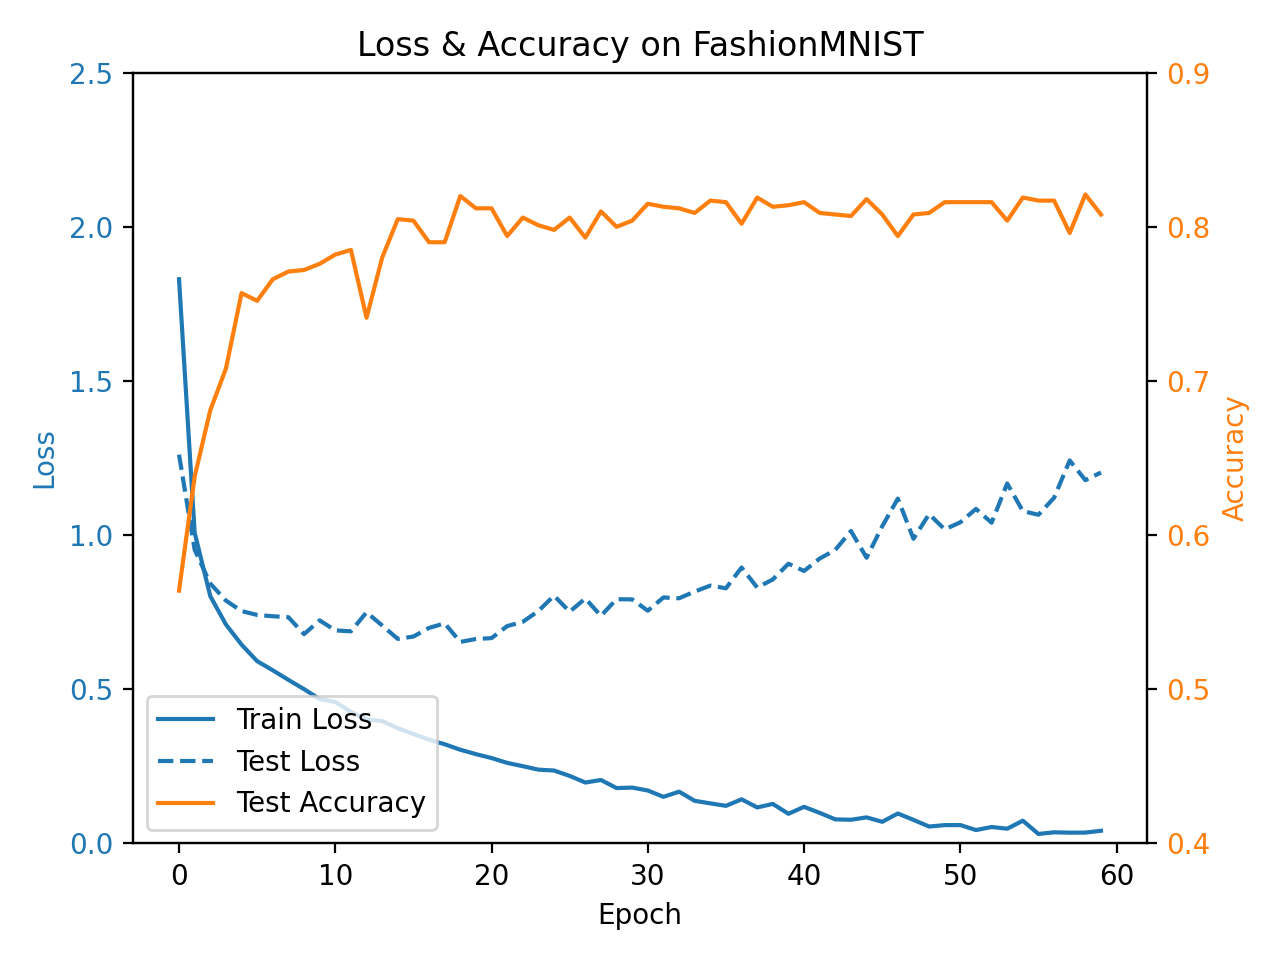
\includegraphics[width=1\textwidth]{plot.png}\\
    \caption{basic torch}
    \label{fig:basic torch}
\end{figure} 

(2).缓解过拟合:\\
\textbf{方法一:Dropout}\\
1.大致实现:引入torch中的dropout方法,在每一轮之后forward之后进行一下dropout,从而缓解过拟合。并进行调参,看最终结果,我试过了一些dropout的参数,发现效果最好在0.4(dropout 参数)左右:\\
2.展示:
\begin{figure}[H]
    \centering
    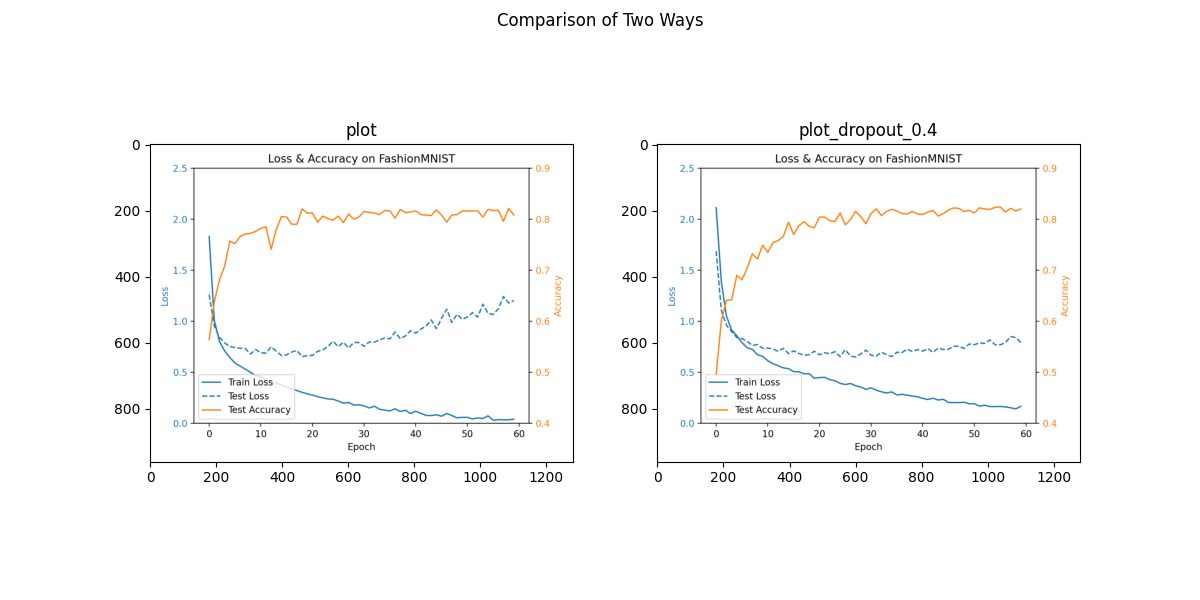
\includegraphics[width=1.1\textwidth]{compare.png}\\
    \caption{basic torch compare with torch with dropout}
    \label{fig:basic torch compare with torch with dropout}
\end{figure} 
3.分析:\\
结合图片我们可以看到,相较于以前的这个testloss都到1以上了,这里的testloss一直后面控制的1以下,而且还保证了最终的训练loss和精度都跟原来区别不大,所以这个方法是有用的.这个方法有用的原因是通过将一部分神经元的输出置为零,通过在训练时随机关闭神经元,dropout 使得网络不能够过于依赖特定的神经元,从而迫使网络学习到更加鲁棒的特征表示,提高了网络的泛化能力,使其对未见过的数据更具有预测能力。\\

\textbf{方法二:模型正则化,权重衰减}\\
1.大致实现:引入torch中的torch.optim as optim方法,实现就是在self中引入了一个sgd的权重衰减\\
2.展示:
\begin{figure}[H]
    \centering
    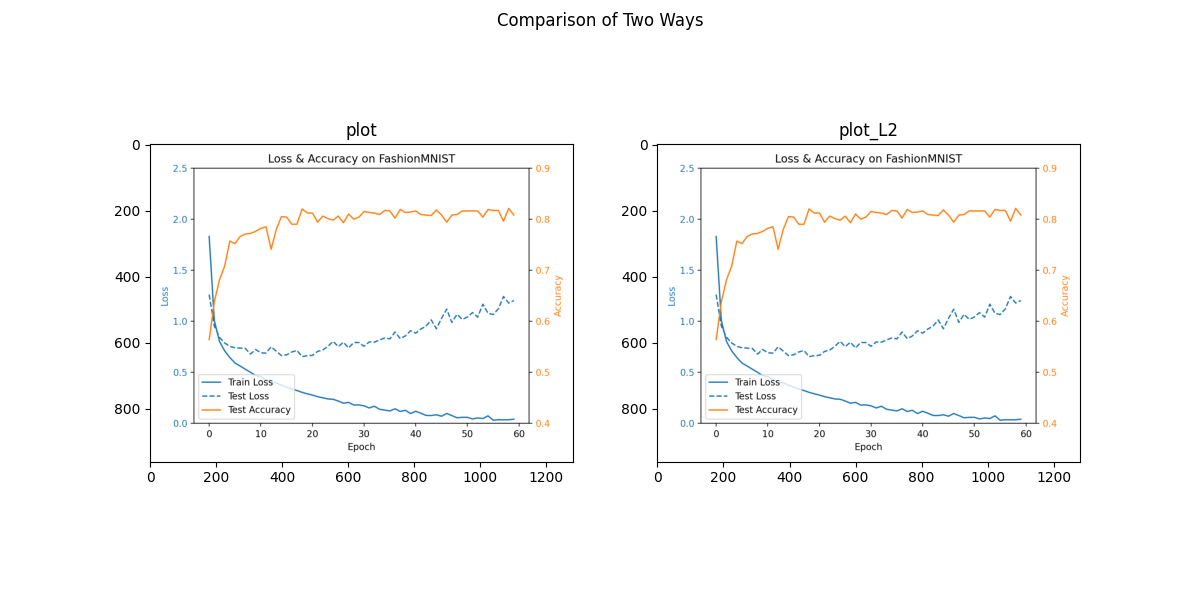
\includegraphics[width=1.1\textwidth]{compare1.png}\\
    \caption{basic torch compare with torch with $weight\_decay$}
    \label{fig:basic torch compare with torch with weight_decay}
\end{figure} 
3.分析:\\
结合图片我们可以看到,好像这种方法并不能缓解过拟合现象,两张图最后都出现了不小的过拟合现象,这使得我们需要调参,但问题是我调过了接近十组参数,发现都不能有效的解决这个过拟合现象,说明现在的这个方法无效。关于这个方法为什么没有用呢,我觉得
可能是训练数据分布不平衡或者噪声相对较少,权重衰减可能会削弱模型对真实信号的学习能力,而更多地惩罚正常的权重。这样可能导致模型性能下降,从而达不到我要的效果。\\

(3)附加题,已在代码中实现。



\end{solution}

\newpage

\section*{Acknowledgments}
允许与其他同样未完成作业的同学讨论作业的内容, 但需在此注明并加以致谢; 如在作业过程中, 参考了互联网上的资料, 且对完成作业有帮助的, 亦需注明并致谢.

\end{document}